\documentclass[11pt,a4paper,oneside,openany]{book}
\usepackage{fontspec}
\usepackage{xeCJK}
\setmainfont{Latin Modern Roman}
\setsansfont{Latin Modern Sans}
\setmonofont{Latin Modern Mono}[Scale=MatchLowercase]
\setCJKmainfont{FandolSong-Regular.otf}[BoldFont=FandolSong-Bold.otf,ItalicFont=FandolKai-Regular.otf]
\setCJKsansfont{FandolHei-Regular.otf}[BoldFont=FandolHei-Bold.otf]
\setCJKmonofont{FandolFang-Regular.otf}
\usepackage[a4paper,inner=23mm,outer=23mm,top=24mm,bottom=24mm,headheight=15pt]{geometry}
\usepackage{amsmath,amssymb,amsthm,bm,mathtools}
\usepackage{graphicx,booktabs,tabularx,array,longtable}
\usepackage{enumitem}
\usepackage{float}
\usepackage{xcolor}
\definecolor{CourseNavy}{HTML}{17324D}
\definecolor{CourseTeal}{HTML}{147D85}
\definecolor{CoursePale}{HTML}{F0F6F8}
\definecolor{CourseGray}{HTML}{536171}
\usepackage{titlesec}
\usepackage{setspace}
\setstretch{1.20}
\setlength{\parindent}{2em}
\setlength{\parskip}{0.25em}
\setlength{\emergencystretch}{2em}
\setlist{nosep,leftmargin=2em,topsep=0.4em}
\setlist[enumerate,1]{label=\arabic*.}
\usepackage[most]{tcolorbox}
\newtcolorbox{coursebox}[1]{enhanced,breakable,colback=CoursePale,colframe=CourseTeal,
  boxrule=0.45pt,arc=1mm,left=3mm,right=3mm,top=2mm,bottom=2mm,
  title={#1},fonttitle=\bfseries\sffamily,coltitle=white,
  before skip=1em,after skip=1em}
\titleformat{\chapter}[display]{\sffamily\bfseries\color{CourseNavy}\huge}
  {\large 第\thechapter 讲}{0.6em}{}
\titlespacing*{\chapter}{0pt}{-10pt}{20pt}
\titleformat{\section}{\Large\sffamily\bfseries\color{CourseNavy}}{\thesection}{0.6em}{}
\titleformat{\subsection}{\large\sffamily\bfseries\color{CourseTeal}}{\thesubsection}{0.6em}{}
\titleformat{\subsubsection}{\normalsize\sffamily\bfseries}{\thesubsubsection}{0.6em}{}
\setcounter{secnumdepth}{2}
\setcounter{tocdepth}{1}
\theoremstyle{definition}
\newtheorem{definition}{定义}[chapter]
\newtheorem{example}{例题}[chapter]
\newtheorem{exercise}{习题}[chapter]
\theoremstyle{plain}
\newtheorem{theorem}{定理}[chapter]
\newtheorem{proposition}[theorem]{命题}
\newtheorem{lemma}[theorem]{引理}
\newtheorem{corollary}[theorem]{推论}
\theoremstyle{remark}
\newtheorem{remark}{说明}[chapter]
\renewcommand{\proofname}{证明}
\newcommand{\R}{\mathbb R}
\newcommand{\E}{\mathbb E}
\DeclareMathOperator{\Var}{Var}
\DeclareMathOperator{\Cov}{Cov}
\DeclareMathOperator{\diag}{diag}
\DeclareMathOperator{\tr}{tr}
\DeclareMathOperator{\rank}{rank}
\DeclareMathOperator*{\argmin}{arg\,min}
\DeclareMathOperator*{\argmax}{arg\,max}
\newcommand{\norm}[1]{\left\lVert#1\right\rVert}
\newcommand{\inner}[2]{\left\langle#1,#2\right\rangle}
\usepackage[numbers,sort&compress]{natbib}
\usepackage{url}
\usepackage[unicode,colorlinks=true,linkcolor=CourseNavy,citecolor=CourseTeal,urlcolor=CourseTeal,
  bookmarksnumbered=true,pdfauthor={冯恺睿},pdftitle={凸优化与非线性优化：2027讲义}]{hyperref}
\usepackage{bookmark}
\usepackage{fancyhdr}
\pagestyle{fancy}
\fancyhf{}
\fancyhead[L]{\small\sffamily\color{CourseGray}凸优化与非线性优化}
\fancyhead[R]{\small\sffamily\color{CourseGray}2027 讲义}
\fancyfoot[C]{\small\thepage}
\renewcommand{\headrulewidth}{0.3pt}
\fancypagestyle{plain}{\fancyhf{}\fancyfoot[C]{\small\thepage}\renewcommand{\headrulewidth}{0pt}}
\renewcommand{\contentsname}{目录}
\renewcommand{\bibname}{参考文献}
\renewcommand{\figurename}{图}
\renewcommand{\tablename}{表}
\newcommand{\coursecover}[3]{%
  \hypersetup{pageanchor=false}
  \begin{titlepage}
  \setlength{\parindent}{0pt}
  \thispagestyle{empty}
  \vspace*{15mm}
  {\sffamily\color{CourseTeal}\Large 2027 \quad COURSE NOTES\par}
  \vspace{12mm}
  {\sffamily\bfseries\color{CourseNavy}\fontsize{31}{42}\selectfont 凸优化与\\非线性优化\par}
  \vspace{7mm}
  {\sffamily\color{CourseGray}\Large Convex and Nonlinear Optimization\par}
  \vspace{13mm}
  {\color{CourseTeal}\rule{\textwidth}{1.1pt}\par}
  \vspace{8mm}
  {\sffamily\bfseries\color{CourseNavy}\LARGE #1\par}
  \vspace{6mm}
  {\large #2\par}
  \vspace{12mm}
  {\normalsize #3\par}
  \vfill
  {\large 主讲：冯恺睿\par}
  \vspace{3mm}
  {\small 同济大学／上海创智学院课程材料\par}
  \vspace{5mm}
  {\small\color{CourseGray}从最优性条件、下降方法与随机噪声，到神经网络的更新几何与参数化。\par}
  \end{titlepage}
  \hypersetup{pageanchor=true}
}

\begin{document}
\coursecover{第1讲：凸优化与下降方法}{4学时理论}{从建模、凸性与光滑性出发，推导梯度下降、Newton方法及预条件的作用。}
\tableofcontents
\chapter{凸优化与下降方法}
\label{l1:chapter}

\begin{coursebox}{本讲目标与课堂安排}
本讲用同一个问题贯穿建模、收敛分析和算法设计：给定数据后，目标函数的几何结构怎样决定一次更新的方向、允许的步长以及最终选中的解？完成本讲后，应能区分凸性、光滑性与强凸性，独立证明梯度下降的基本收敛界，说明 Newton 法为什么需要阻尼，并计算欠定最小二乘中梯度下降的极限。

本讲安排为四个理论学时。按每学时45分钟，可依次分配为：建模与凸性35分钟，光滑性与梯度下降55分钟，线搜索与 Newton 法40分钟，预条件与最小范数50分钟。标为“选读”的证明和练习不要求全部在课堂完成。课堂必须掌握的是定理的假设、证明中起作用的不等式，以及结论不能覆盖的情形。
\end{coursebox}

\section{从学习问题到优化问题}
\label{l1:modeling}

设训练数据为 $\{(a_i,y_i)\}_{i=1}^n$，模型参数为 $x\in\R^d$，模型预测为 $F_x(a)$。一个常见的训练目标是
\begin{equation}
    \min_{x\in C} f(x),\qquad
    f(x)=\frac1n\sum_{i=1}^n\ell(F_x(a_i),y_i)+\lambda R(x),
    \label{l1:erm}
\end{equation}
其中 $C$ 表示可行集合，$R$ 表示显式正则项，$\lambda\geq0$。本讲先取 $C=\R^d$，第二讲再处理约束。不要把数据、模型和优化器混成一个对象：数据与模型共同决定 $f$，优化器根据 $f$ 或其随机估计生成迭代，而泛化误差还涉及训练分布与测试分布之间的关系。

即使损失 $\ell(z,y)$ 对预测值 $z$ 是凸函数，复合函数 $x\mapsto\ell(F_x(a),y)$ 也未必对参数凸。线性预测 $F_x(a)=a^\top x$ 保持许多常用损失的凸性；神经网络中参数相乘、非线性激活与层间组合通常破坏这一结构。我们先学习凸模型，是为了获得可以逐步检查的参照系，随后才讨论哪些论证仍能用于非凸训练。

以下默认 $\inner{u}{v}=u^\top v$，$\norm{x}$ 为 Euclidean 范数，矩阵范数 $\norm{A}_2$ 为算子范数。对称矩阵 $H\succeq0$ 表示 $v^\top Hv\geq0$ 对所有 $v$ 成立。记最优值为 $f^*=\inf_x f(x)$；只有确认最小值取到以后，才写 $x^*\in\argmin f$。

\subsection{先问存在性，再问算法}

“损失有下界”并不意味着“存在有限参数的最优解”。例如 $f(x)=e^x$ 的下确界是0，但没有任何有限 $x$ 使它等于0。相反，若 $f$ 连续，而且某个非空下水平集 $\{x:f(x)\leq f(x_0)\}$ 紧，则在该集合上存在最小值。强凸函数若在整个 $\R^d$ 上有限且连续，则其二次下界保证强制性，从而存在唯一最小点。

这一区分会影响停止准则。参数不断增大时，损失可能仍在下降；损失下降缓慢也可能只是目标在某些方向很平坦。观察一条 loss 曲线不足以判断目标是否存在、算法是否稳定或模型是否泛化。

\begin{example}[最小二乘与岭回归的建模]
\label{l1:ex-ridge}
将样本特征堆叠为 $A\in\R^{n\times d}$，标签为 $b\in\R^n$。为减少不必要的常数，考虑
\[
 f_\lambda(x)=\frac12\norm{Ax-b}^2+\frac\lambda2\norm{x}^2.
\]
本节使用未平均的数据项。若把整个目标除以 $n$，梯度与光滑常数都相应除以 $n$，正则系数也变为 $\lambda/n$。若代码仅对数据项取均值，采用 $\norm{Ax-b}^2/(2n)+\lambda\norm{x}^2/2$，则梯度为 $A^\top(Ax-b)/n+\lambda x$，Hessian 为 $A^\top A/n+\lambda I$，不能把正则项也自动除以 $n$。因此损失归一化、正则系数和学习率应一起注明。对本例所写的未平均目标，直接求导得
\[
 \nabla f_\lambda(x)=A^\top(Ax-b)+\lambda x,
 \qquad H=A^\top A+\lambda I.
\]
当 $\lambda>0$ 时，$H\succeq\lambda I$，唯一解为
\[
 x_\lambda=(A^\top A+\lambda I)^{-1}A^\top b.
\]
公式中的逆矩阵是数学表达，实际计算一般解线性方程，不显式求逆。

取 $A=\diag(1,3)$，$b=(1,3)^\top$。无正则化时，$H=\diag(1,9)$，最优点为 $(1,1)^\top$。当 $\lambda=1$ 时，最优点变为 $(1/2,9/10)^\top$，Hessian 变为 $\diag(2,10)$。条件数从9降到5，但优化目标也改变了。因此，“加入正则项使优化更容易”与“保持原问题、只改进求解方法”是两件不同的事。
\end{example}

\section{凸性、光滑性与强凸性分别控制什么}
\label{l1:geometry}

\subsection{凸集、凸函数与一阶判据}

\begin{definition}[凸集与凸函数]
集合 $C\subseteq\R^d$ 是凸集，如果对任意 $x,y\in C$ 与 $t\in[0,1]$，都有 $(1-t)x+ty\in C$。函数 $f:C\to\R$ 是凸函数，如果
\[
 f((1-t)x+ty)\leq(1-t)f(x)+tf(y).
\]
当 $x\ne y$、$t\in(0,1)$ 时严格小于成立，则称为严格凸。
\end{definition}

仿射子空间、半空间、范数球和它们的交集都是凸集。凸函数的非负加权和仍然凸，与仿射映射复合也保持凸性。这些规则使我们能够从简单模块识别一个模型，而不必每次计算完整 Hessian。凸性提供的是全局几何信息：任意局部极小点都是全局极小点。严格凸性保证极小点至多一个，却不保证极小点一定存在。

\begin{proposition}[可微凸函数的一阶刻画]
\label{l1:prop-convex-first}
设 $f$ 在包含凸集 $C$ 的开集上可微。则 $f$ 在 $C$ 上凸，当且仅当对任意 $x,y\in C$ 有
\begin{equation}
 f(y)\geq f(x)+\inner{\nabla f(x)}{y-x}.
 \label{l1:first-order-convex}
\end{equation}
特别地，对整个 $\R^d$ 上的可微凸函数，$\nabla f(x^*)=0$ 当且仅当 $x^*$ 是全局极小点。
\end{proposition}

\begin{proof}
若 $f$ 凸，令 $z_t=x+t(y-x)$。凸性给出
\[
 \frac{f(z_t)-f(x)}t\leq f(y)-f(x).
\]
令 $t\downarrow0$ 即得\eqref{l1:first-order-convex}。反过来，令 $z=(1-t)x+ty$，分别在 $z$ 处对 $x,y$ 使用一阶下界，再以权重 $1-t,t$ 相加，梯度项相消，得到凸性不等式。无约束最优点的梯度为零来自可微函数的一阶必要条件；凸性则使该条件充分。
\end{proof}

若 $f$ 二阶连续可微，则在开凸域上，$f$ 凸等价于 $\nabla^2f(x)\succeq0$ 对域内所有 $x$ 成立。这里的“所有点”不能换成“当前点”。例如 $f(x)=x^4-x^2$ 在足够远处 Hessian 为正，但整个函数并不凸。对非凸目标，$\nabla f=0$ 可能对应局部极小、局部极大或鞍点。

\subsection{上曲率界与下曲率界}

\begin{definition}[光滑与强凸]
可微函数 $f$ 是 $L$-光滑的，如果
\[
 \norm{\nabla f(x)-\nabla f(y)}\leq L\norm{x-y}.
\]
它是 $\mu$-强凸的，如果 $\mu>0$ 且
\begin{equation}
 f(y)\geq f(x)+\inner{\nabla f(x)}{y-x}
             +\frac\mu2\norm{y-x}^2.
 \label{l1:strong-convex}
\end{equation}
当两者同时成立时，定义条件数 $\kappa=L/\mu$。
\end{definition}

光滑性限制梯度变化的速度，所以约束允许的步长；强凸性限制目标在最优点附近有多平，所以有助于控制误差的消除速度。若 $f$ 二阶连续可微且凸，则
\[
 \mu I\preceq\nabla^2f(x)\preceq LI
\]
是同时刻画强凸与光滑的 Hessian 条件。对非凸光滑函数，上述光滑性对应 $\norm{\nabla^2f(x)}_2\leq L$，允许负特征值存在。

强凸性比严格凸性强。$x^4$ 在实线上严格凸，但在0处没有正的二次曲率下界；它也不是整个实线上的 $L$-光滑函数，因为二阶导数 $12x^2$ 无界。在有界区间上又可以给出局部光滑常数。因此，报告一个 $L$ 时应说明适用区域。

\begin{lemma}[下降引理]
\label{l1:lemma-descent}
若 $f$ 在包含线段 $[x,y]$ 的区域上具有 $L$-Lipschitz 梯度，则
\begin{equation}
 f(y)\leq f(x)+\inner{\nabla f(x)}{y-x}
                 +\frac L2\norm{y-x}^2.
 \label{l1:descent-lemma}
\end{equation}
该结论不要求 $f$ 凸。
\end{lemma}

\begin{proof}
令 $d=y-x$，由微积分基本定理，
\begin{align*}
 f(y)-f(x)-\inner{\nabla f(x)}d
 &=\int_0^1\inner{\nabla f(x+td)-\nabla f(x)}d\,dt\\
 &\leq\int_0^1 Lt\norm d^2\,dt
 =\frac L2\norm d^2.
\end{align*}
\end{proof}

下降引理把复杂目标替换成一个容易最小化的局部二次上界。强凸性给的是二次下界，二者的方向相反。之后的算法分析反复使用这两个模型，而不是直接展开原目标的所有项。

\begin{proposition}[强凸情形的误差证书]
\label{l1:prop-gap}
若 $f$ 可微、$\mu$-强凸，并有最优点 $x^*$，则
\begin{equation}
 \frac\mu2\norm{x-x^*}^2
 \leq f(x)-f^*
 \leq\frac{\norm{\nabla f(x)}^2}{2\mu}.
 \label{l1:gap-gradient}
\end{equation}
\end{proposition}

\begin{proof}
左边是在 $x^*$ 处使用强凸下界和 $\nabla f(x^*)=0$。对右边，在任意 $x$ 处的强凸下界中令 $y=x^*$，再利用
\[
 \inner{g}{y-x}+\frac\mu2\norm{y-x}^2
 \geq-\frac{\norm g^2}{2\mu}
\]
即可。
\end{proof}

\section{梯度下降：从一步下降到收敛速率}
\label{l1:gd}

考虑迭代
\begin{equation}
 x_{t+1}=x_t-\eta\nabla f(x_t),\qquad \eta>0.
 \label{l1:gd-update}
\end{equation}
它也可写成二次局部模型的最小点：
\[
 x_{t+1}=\argmin_z
 \left\{\inner{\nabla f(x_t)}{z-x_t}
       +\frac1{2\eta}\norm{z-x_t}^2\right\}.
\]
这个表达揭示了 Euclidean 几何的作用：算法以参数位移的平方范数惩罚过大的更新。后面改变这一惩罚，就会得到预条件方法。

\subsection{一步下降不等式}

将\eqref{l1:gd-update}代入下降引理，得到
\begin{equation}
 f(x_{t+1})\leq f(x_t)
 -\eta\left(1-\frac{L\eta}{2}\right)\norm{\nabla f(x_t)}^2.
 \label{l1:gd-descent}
\end{equation}
当 $0<\eta<2/L$ 时，非零梯度保证严格下降。这个结论适用于非凸函数，但不意味着一定到达全局最小值。若 $f$ 有下界且步长固定，求和可控制梯度平方的总量；第三讲将把它扩展为带随机梯度噪声的驻点收敛界。

还应区分“充分稳定步长”与“最优步长”。$1/L$ 的优点是推导简单且有统一保证，不表示它对每一个目标、初始化或计算预算都最优。用某个模型得到的最佳常数，也不能直接搬到一般神经网络上。

\subsection{凸但不强凸：函数值的 $O(1/T)$ 界}

\begin{theorem}[光滑凸梯度下降]
\label{l1:thm-gd-convex}
设 $f:\R^d\to\R$ 凸、$L$-光滑，且存在最优点 $x^*$。取固定步长 $0<\eta\leq1/L$，则对 $T\geq1$，
\begin{equation}
 f(x_T)-f^*\leq\frac{\norm{x_0-x^*}^2}{2\eta T}.
 \label{l1:gd-convex-rate}
\end{equation}
\end{theorem}

\begin{proof}
记 $g_t=\nabla f(x_t)$。凸性和下降引理共同给出
\begin{align*}
 f(x_{t+1})-f^*
 &\leq\inner{g_t}{x_t-x^*}
       -\eta\left(1-\frac{L\eta}{2}\right)\norm{g_t}^2.
\end{align*}
另一方面，展开距离有
\[
 \norm{x_t-x^*}^2-\norm{x_{t+1}-x^*}^2
 =2\eta\inner{g_t}{x_t-x^*}-\eta^2\norm{g_t}^2.
\]
因此
\begin{align}
 f(x_{t+1})-f^*
 &\leq\frac{\norm{x_t-x^*}^2-\norm{x_{t+1}-x^*}^2}{2\eta}
 -\frac\eta2(1-L\eta)\norm{g_t}^2\\
 &\leq\frac{\norm{x_t-x^*}^2-\norm{x_{t+1}-x^*}^2}{2\eta}.
 \label{l1:gd-telescope}
\end{align}
对 $t=0,\ldots,T-1$ 求和，右侧望远镜相消。又因函数值单调不增，左侧不小于 $T(f(x_T)-f^*)$，得到结论。
\end{proof}

这个证明值得完整掌握。它的三个部件是：凸性把目标差转成梯度内积，平方距离恒等式把内积转成势函数差，最后通过求和得到速率。投影梯度与近端梯度的分析会沿用同一种结构，只是需要额外的最优性条件。

当 $\eta=1/L$ 时，要保证 $f(x_T)-f^*\leq\epsilon$，上界要求 $T\geq L\norm{x_0-x^*}^2/(2\epsilon)$。这里的 $O(1/T)$ 描述目标差，不是说参数距离必然也按 $1/T$ 下降，更不是运行时间一定只由 $T$ 决定；每步的梯度计算成本也要计入。

\subsection{强凸：线性收敛}

\begin{theorem}[光滑强凸梯度下降]
\label{l1:thm-gd-strong}
设 $f:\R^d\to\R$ 为 $L$-光滑且 $\mu$-强凸。取 $\eta=1/L$，则
\begin{equation}
 f(x_T)-f^*\leq
 \left(1-\frac\mu L\right)^T\bigl(f(x_0)-f^*\bigr).
 \label{l1:gd-strong-rate}
\end{equation}
\end{theorem}

\begin{proof}
一步下降式给出
\[
 f(x_{t+1})-f^*
 \leq f(x_t)-f^*-\frac1{2L}\norm{\nabla f(x_t)}^2.
\]
利用\eqref{l1:gap-gradient}中的梯度下界
$\norm{\nabla f(x_t)}^2\geq2\mu(f(x_t)-f^*)$，便得到收缩因子 $1-\mu/L$。反复迭代即可。
\end{proof}

“线性收敛”指误差被固定比例压缩，也称几何或指数收敛，并不是误差与迭代次数成线性函数。当 $\kappa=L/\mu$ 大时，$1-1/\kappa$ 接近1，所以需要约 $O(\kappa\log(1/\epsilon))$ 次迭代。该量级说明提高精度与改善条件数是不同问题：前者进入对数项，后者直接影响收敛常数。

\subsection{二次函数的精确谱分析}

令
\[
 f(x)=\frac12(x-x^*)^\top H(x-x^*)+f^*,
 \qquad H=Q\Lambda Q^\top\succ0.
\]
取误差 $e_t=x_t-x^*$，在特征坐标 $z_t=Q^\top e_t$ 下，
\begin{equation}
 e_{t+1}=(I-\eta H)e_t,
 \qquad z_{t+1,i}=(1-\eta\lambda_i)z_{t,i}.
 \label{l1:quad-mode}
\end{equation}
每个特征方向都是一条独立的一阶递推。所有初始化均收敛的充要条件为
\[
 0<\eta<\frac2{\lambda_{\max}(H)}.
\]
记 $\mu=\lambda_{\min}(H)$、$L=\lambda_{\max}(H)$，最坏方向的误差因子是
\[
 q(\eta)=\max_i|1-\eta\lambda_i|
        =\max\{|1-\eta\mu|,|1-\eta L|\}.
\]
平衡两端可得该二次模型下最优固定步长与因子
\begin{equation}
 \eta_{\rm quad}=\frac2{L+\mu},
 \qquad q_{\rm quad}=\frac{L-\mu}{L+\mu}
                    =\frac{\kappa-1}{\kappa+1}.
 \label{l1:quad-optimal-step}
\end{equation}
这是针对全部初始化的最坏方向而言。某个特定初始化若完全没有落在慢方向上，可以更快。目标差的收缩因子是 $q^2$，参数范数的因子是 $q$，书写时不要漏掉平方。

\begin{example}[同一目标下的三种步长]
\label{l1:ex-gd-spectrum}
回到例\ref{l1:ex-ridge}的无正则化目标，$H=\diag(1,9)$。令 $x_0-x^*=(3,1)^\top$，初始目标差为9。

取 $\eta=1/9$，两个方向的因子分别是 $8/9$ 与0，所以
\[
 e_t=\bigl(3(8/9)^t,0\bigr)^\top\quad(t\geq1),\qquad
 f(x_t)-f^*=\frac92(8/9)^{2t}.
\]
取 $\eta=1/5=2/(1+9)$，因子变为 $4/5$ 与 $-4/5$，于是
\[
 e_t=\bigl(3(4/5)^t,(-4/5)^t\bigr)^\top,
 \qquad f(x_t)-f^*=9(16/25)^t.
\]
第二个坐标来回变号，但振幅衰减，所以振荡不等于发散。若希望目标差降至初始值的1\%，这两种步长分别需要至少17步和11步。

取 $\eta=1/4$ 时，最大曲率方向的因子为 $-5/4$，只要初始误差在该方向非零就发散。该例说明：慢方向希望更大的步长，快方向限制最大步长；条件数正是两者冲突的程度。
\end{example}

\begin{figure}[htbp]
\centering
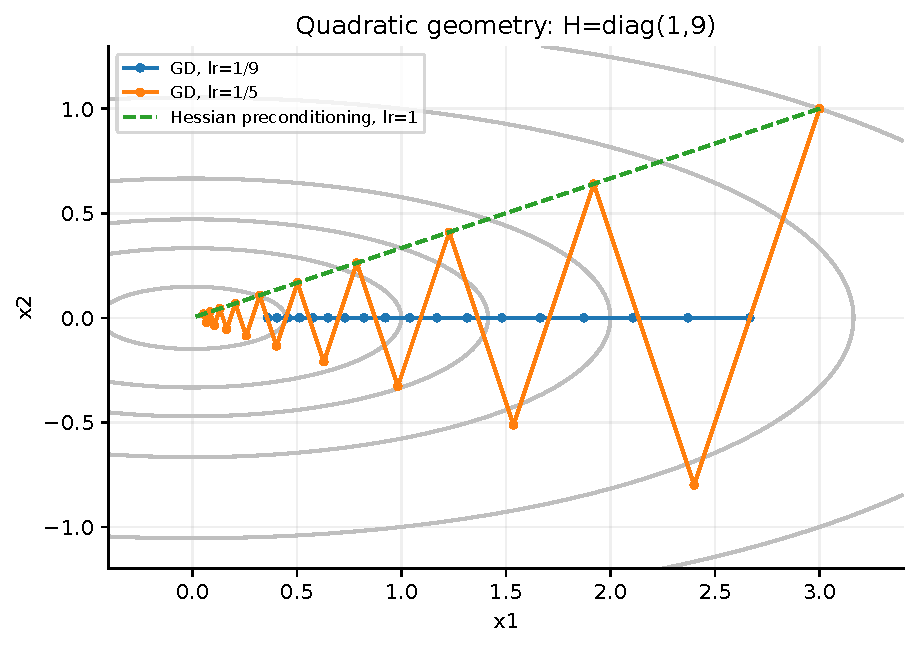
\includegraphics[width=0.85\textwidth]{figures/quadratic_geometry.pdf}
\caption{二次目标 $f(x)-f^*=\tfrac12e^\top He$ 的下降几何，其中 $e=x-x^*$、$H=\diag(1,9)$、$e_0=(3,1)^\top$。步长 $\eta=1/9$ 一步消除高曲率方向的误差，随后沿低曲率方向缓慢前进；$\eta=1/5$ 使两个方向的收缩幅度同为 $4/5$，高曲率坐标交替变号但振幅衰减。使用 Hessian 逆预条件 $P=H^{-1}$ 时，有效 Hessian 为单位阵，单位步长可一步消除该二次模型的误差。}
\label{l1:fig-quadratic-geometry}
\end{figure}

\section{不知道光滑常数时：回溯线搜索}
\label{l1:line-search}

实际问题中，全局 $L$ 可能难以估计，也可能比当前区域的曲率大很多。回溯线搜索利用已计算的梯度，试探一个足够下降的步长。设 $d_t$ 满足 $\inner{\nabla f(x_t)}{d_t}<0$，选择 $c\in(0,1)$、$\beta\in(0,1)$ 和初始试探步长 $\alpha_0>0$。从 $\alpha=\alpha_0$ 开始，若
\begin{equation}
 f(x_t+\alpha d_t)
 \leq f(x_t)+c\alpha\inner{\nabla f(x_t)}{d_t}
 \label{l1:armijo}
\end{equation}
不成立，就令 $\alpha\leftarrow\beta\alpha$ 并重试。接受后设置 $x_{t+1}=x_t+\alpha d_t$。式\eqref{l1:armijo}称为 Armijo 充分下降条件；它比较实际下降与一阶模型预测下降的一定比例\citep{Nocedal2006}。

\begin{proposition}[回溯何时有限终止]
\label{l1:prop-backtracking}
若 $\nabla f(x_t)^\top d_t<0$，且试探线段附近梯度为 $L$-Lipschitz，则任意满足
\[
 0<\alpha\leq
 \frac{-2(1-c)\inner{\nabla f(x_t)}{d_t}}{L\norm{d_t}^2}
\]
的步长都满足 Armijo 条件。因此，几何回溯会有限终止。对 $d_t=-\nabla f(x_t)$，充分条件简化为 $\alpha\leq2(1-c)/L$。
\end{proposition}

\begin{proof}
下降引理给出
\[
 f(x_t+\alpha d_t)
 \leq f(x_t)+\alpha\inner{g_t}{d_t}
       +\frac{L\alpha^2}{2}\norm{d_t}^2.
\]
要求右侧不超过 $f(x_t)+c\alpha\inner{g_t}{d_t}$，整理即得。
\end{proof}

线搜索并非免费：一次梯度更新可能需要多次目标评估。对全批量问题，这常是合理成本；对随机 mini-batch，若每次试探都更换数据，比较的就不再是同一个函数，以上结论不能直接使用。算法理论中的一个“迭代步”与实验中的一次前向、一次反向、一次数据遍历必须区分。

停止准则也要说明能证明什么。在强凸情形，$\norm{\nabla f(x)}\leq\varepsilon$ 给出目标差不超过 $\varepsilon^2/(2\mu)$。一般非凸情形，小梯度只是一阶驻点证据。单独使用“连续两步损失变化很小”不可靠：步长过小也会产生这一现象。实际可联合检查梯度、步长、目标变化和预算，并记录它们各自的量纲。

\section{Newton 法：利用曲率，也检验曲率}
\label{l1:newton}

\subsection{二次局部模型与下降方向}

设 $f$ 二阶可微，$g_t=\nabla f(x_t)$、$H_t=\nabla^2f(x_t)$。Newton 法在当前点使用模型
\[
 m_t(d)=f(x_t)+\inner{g_t}d+\frac12d^\top H_td.
\]
当 $H_t\succ0$ 时，该模型唯一极小点解方程
\begin{equation}
 H_td_t=-g_t,
 \qquad x_{t+1}=x_t+\alpha_td_t.
 \label{l1:newton-step}
\end{equation}
而且 $g_t^\top d_t=-g_t^\top H_t^{-1}g_t<0$，所以非零梯度下它是下降方向。对严格凸二次目标，Hessian 不随位置改变，取 $\alpha_t=1$ 一步到达最优点。

这并不意味着 Newton 法总比梯度下降快。每步需要表示或近似曲率、求解线性系统；在高维学习问题中，这些成本可能显著。更关键的是，远离最优点时二次模型可能不准确，非凸 Hessian 还可能不正定。一个求解了线性方程的向量，不一定是原目标的下降方向。

\begin{example}[步长阻尼与 Hessian 修正处理不同问题]
\label{l1:ex-newton}
先看凸函数 $f(x)=e^x-x$，唯一最优点为0。Newton 方向为
\[
 d(x)=-\frac{e^x-1}{e^x}=e^{-x}-1.
\]
从 $x_0=-2$ 出发，$d_0=e^2-1\approx6.389$。全步长到达 $x_1\approx4.389$，函数值从约2.135增至约76.2。方向本身是下降方向，但走得过远，二次近似失效。

取 Armijo 参数 $c=0.1$、回缩因子 $\beta=1/2$。试探 $\alpha=1$ 失败；$\alpha=1/2$ 时函数值约2.107，仍未达到所要求的充分下降；$\alpha=1/4$ 时到达约 $-0.403$，函数值约1.071，满足条件。这是通过缩短步长来控制模型误差。

再看非凸函数 $h(x)=x^4/4-x^2/2$。在 $x=0.1$，有 $h'(x)=-0.099$、$h''(x)=-0.97$，Newton 方向约为 $-0.1021$，与梯度内积为正。此时方向向局部极大点0移动，任意足够小的正步长都会上升。仅做步长回缩无法把上升方向变成下降方向；必须先修正曲率模型或更换方向。
\end{example}

一种曲率修正是求解
\[
 (H_t+\tau_t I)d_t=-g_t,
 \qquad H_t+\tau_t I\succ0,
\]
再配合线搜索。这里 $\tau_t$ 改变方向，$\alpha_t$ 改变沿该方向走多远。二者有不同职责。还可以使用信赖域，直接限制二次模型的可信区域；其完整理论留作\citet{Nocedal2006}的延伸阅读。

\subsection{选读：局部二次收敛的准确条件}

\begin{theorem}[Newton 法的局部误差界]
\label{l1:thm-newton-local}
设 $\nabla f(x^*)=0$。在以 $x^*$ 为中心的某个凸邻域中，假设
\[
 \nabla^2f(x)\succeq\mu I\quad(\mu>0),\qquad
 \norm{\nabla^2f(x)-\nabla^2f(y)}_2\leq M\norm{x-y}.
\]
若当前点 $x_t$ 位于该邻域，Newton 全步的误差满足
\begin{equation}
 \norm{x_{t+1}-x^*}\leq\frac{M}{2\mu}\norm{x_t-x^*}^2.
 \label{l1:newton-quadratic}
\end{equation}
若初始点足够近，使上述误差界保证后续点始终留在邻域内，则全步 Newton 法局部二次收敛。
\end{theorem}

\begin{proof}
令 $e_t=x_t-x^*$，由梯度的积分表达式，
\[
 g_t=\int_0^1\nabla^2 f(x^*+se_t)e_t\,ds.
\]
因此
\[
 e_{t+1}=H_t^{-1}\int_0^1
 \bigl[H_t-\nabla^2f(x^*+se_t)\bigr]e_t\,ds.
\]
利用 $\norm{H_t^{-1}}_2\leq1/\mu$ 与 Hessian 的 Lipschitz 条件，积分上界为
\[
 \frac1\mu\int_0^1M(1-s)\norm{e_t}^2\,ds
 =\frac{M}{2\mu}\norm{e_t}^2.
\]
例如选取包含于原邻域、半径不超过 $\mu/M$ 的球，就可由误差至少减半保证迭代不离开该球；$M=0$ 时对应局部精确二次模型。
\end{proof}

“二次收敛”是局部误差递推的阶数，不能解释成对任何初始化都只需很少步，也不能忽略求线性系统的数值误差。精确理论为阻尼策略提供目标：远处先保证进展，进入合适区域后再利用全步的快速收敛。

\section{预条件：改变更新所使用的几何}
\label{l1:preconditioning}

选择对称正定矩阵 $P$，考虑
\begin{equation}
 x_{t+1}=x_t-\eta P\nabla f(x_t).
 \label{l1:precondition-update}
\end{equation}
它恰好是下列局部模型的最小点：
\[
 \argmin_z\left\{\inner{\nabla f(x_t)}{z-x_t}
 +\frac1{2\eta}(z-x_t)^\top P^{-1}(z-x_t)\right\}.
\]
换言之，$P^{-1}$ 定义位移的代价。在某个方向给更小的位移代价，就允许该方向更大的更新。这比“每个坐标分别乘一个学习率”的描述更一般，因为 $P$ 可以包含非对角项。

令 $x=P^{1/2}z$，定义 $\widetilde f(z)=f(P^{1/2}z)$，则\eqref{l1:precondition-update}等价于在 $z$ 坐标对 $\widetilde f$ 做普通梯度下降。若原目标为 Hessian $H\succ0$ 的二次函数，新的 Hessian 是
\begin{equation}
 \widetilde H=P^{1/2}HP^{1/2}.
 \label{l1:precondition-hessian}
\end{equation}
有效条件数应根据这个对称矩阵计算。$PH$ 虽不一定对称，但与它相似，具有相同正特征值。取 $P=H^{-1}$ 时，$\widetilde H=I$；对于大型问题，恰恰是精确构造和应用这个逆矩阵的成本促使我们研究对角、块对角或其他结构近似。

\begin{example}[标准化不等于白化]
\label{l1:ex-whitening}
考虑 $H=\begin{pmatrix}1&\rho\\\rho&1\end{pmatrix}$，$0<\rho<1$。两个坐标的尺度已经相同，对角预条件 $P=\diag(H)^{-1}=I$ 完全不改变问题。然而 $H$ 的特征值是 $1+\rho$ 与 $1-\rho$，条件数为 $(1+\rho)/(1-\rho)$；当 $\rho=0.99$ 时条件数为199。

取完整预条件 $P=H^{-1}$ 则有效条件数为1。这说明差异不仅来自边际尺度，也来自坐标之间的相关性。对数据协方差 $\Sigma$，逐坐标标准化得到的是 $D^{-1}\Sigma D^{-1}$，一般只是对角为1的相关矩阵；只有合适的完整白化才把它变为单位阵。后续讨论 BatchNorm、LayerNorm 或自适应优化器时，不能把它们直接称为精确白化。
\end{example}

预条件也揭示了参数化的意义：同一个预测函数若用不同坐标表示，Euclidean 梯度下降通常产生不同的函数更新。只有同时变换更新所用的几何，才可能保留相同轨迹。第五讲会把这一观察推广到网络 Jacobian 与有效训练核。

\section{欠定最小二乘：优化器会选择哪个解}
\label{l1:min-norm}

设 $A\in\R^{n\times d}$ 非零但可能秩亏，考虑
\[
 \min_x\frac12\norm{Ax-b}^2.
\]
当 $\ker A\ne\{0\}$ 时，目标无法区分沿零空间的参数变化。即使训练预测唯一，参数解也可能有无穷多个。此时我们需要回答两个问题：算法是否收敛，以及收敛到哪一个最优解。

\begin{theorem}[梯度下降的最小范数选择]
\label{l1:thm-min-norm}
设 $A\ne0$，固定步长满足 $0<\eta<2/\norm A_2^2$。对最小二乘目标作梯度下降，则
\begin{equation}
 x_t\longrightarrow A^\dagger b+\Pi_{\ker A}x_0,
 \label{l1:min-norm-limit}
\end{equation}
其中 $A^\dagger$ 是 Moore--Penrose 伪逆，$\Pi_{\ker A}$ 是到 $A$ 零空间的正交投影。特别地，从 $x_0=0$ 出发，极限是所有最小二乘解中 Euclidean 范数最小的解。
\end{theorem}

\begin{proof}
取紧致奇异值分解 $A=U_r\Sigma_rV_r^\top$，其中 $r=\rank A$、$\Sigma_r=\diag(\sigma_1,\ldots,\sigma_r)$ 且 $\sigma_i>0$。每次更新 $-\eta A^\top(Ax_t-b)$ 都在 $\operatorname{range}(A^\top)$ 中，所以零空间分量保持为 $\Pi_{\ker A}x_0$。

在第 $i$ 个右奇异向量方向，记 $z_{t,i}=v_i^\top x_t$，则
\[
 z_{t+1,i}=(1-\eta\sigma_i^2)z_{t,i}
              +\eta\sigma_i u_i^\top b.
\]
步长条件保证 $|1-\eta\sigma_i^2|<1$，其极限为 $u_i^\top b/\sigma_i$。合起来就是 $V_r\Sigma_r^{-1}U_r^\top b=A^\dagger b$。

全部最小二乘解为 $A^\dagger b+v$，$v\in\ker A$。两部分正交，故
\[
 \norm{A^\dagger b+v}^2=\norm{A^\dagger b}^2+\norm v^2.
\]
取 $v=0$ 得到唯一最小范数解。该证明不要求 $Ax=b$ 一致。
\end{proof}

该结论是一个完整的隐式偏置例子：目标函数没有写入 $\norm x^2$ 惩罚，但初始化与更新结构仍选出某一类解。这个选择不等于加入固定强度的岭正则；岭回归通常改变拟合结果，而这里极限仍然精确最小化原始最小二乘损失。

\subsection{预条件怎样改变所选解}

对固定 $P\succ0$，从0出发作预条件梯度下降。通过 $x=P^{1/2}z$ 变换，普通梯度下降在 $z$ 空间选择最小 $\norm z$ 的解，所以在 $x$ 空间选择最小 $x^\top P^{-1}x$ 的最小二乘解。若 $A$ 满行秩，则 $Ax=b$ 总可行，且
\begin{equation}
 x_P=P A^\top(AP A^\top)^{-1}b.
 \label{l1:weighted-min-norm}
\end{equation}
相应稳定步长需要满足 $0<\eta<2/\norm{AP^{1/2}}_2^2$。同样的训练误差不保证同样的参数，也不保证在新输入上给出同样的预测。

\begin{example}[同一条插值直线上的两种选择]
\label{l1:ex-min-norm}
设 $A=(1\ \ 2)$、$b=1$。所有插值解满足 $x_1+2x_2=1$。普通梯度下降从0出发，每步都沿向量 $(1,2)^\top$ 移动，因此极限必为该直线与 $\operatorname{span}(1,2)^\top$ 的交点：
\[
 x_I=\frac15(1,2)^\top=(1/5,2/5)^\top.
\]
取 $P=\diag(4,1)$，更新方向改为 $(4,2)^\top$。由\eqref{l1:weighted-min-norm}，
\[
 x_P=\frac18(4,2)^\top=(1/2,1/4)^\top.
\]
二者都使训练损失为0，但 Euclidean 范数平方分别为 $1/5$ 与 $5/16$。第二个解最小化的是 $x_1^2/4+x_2^2$，其值为 $1/8$，低于第一个解的 $17/100$。若测试输入为 $(1,0)$，两者预测分别为 $1/5$ 与 $1/2$。只看训练损失无法判断哪一个预测更合理，还需要关于数据生成过程的假设。
\end{example}

\section{本讲结论如何进入后续课程}
\label{l1:bridge}

本讲建立了三种不同的判断。第一，凸性与强凸性决定哪些驻点可以作为全局最优证书。第二，光滑常数与条件数解释步长限制和收敛速度。第三，参数空间中的几何与初始化决定在多解问题中选择哪个解。它们之间有关联，但不能互相替代：更快的收敛不自动意味着更好的泛化，更小的梯度也不自动意味着解决了非凸全局优化。

第二讲在约束边界处用 KKT 条件替代无约束的 $\nabla f=0$；第三讲研究梯度含随机误差时哪些递推需要增加噪声项；第四讲比较不同几何下的更新；第五讲把 $P$ 与网络 Jacobian 共同纳入函数空间动力学。建议阅读\citet{Boyd2004}的凸函数与无约束最小化章节、\citet{Nesterov2004}的一阶复杂度分析，以及\citet{Nocedal2006}的线搜索与 Newton 方法。课堂证明已经给出本讲所需的主要结论，延伸阅读用于理解更一般的条件和更强的算法。

\section{习题}
\label{l1:exercises}

\begin{exercise}[基本性质与结论边界]
\label{l1:exercise-properties}
分别判断 $f_1(x)=x^4$、$f_2(x)=e^x$、$f_3(x)=x^2/2$ 在整个实线上是否凸、严格凸、强凸、全局光滑，以及是否存在最优点。再说明：把定义域限制为 $[-1,1]$ 后，哪些光滑性结论发生改变？不要用“图像像碗”代替导数或定义证明。
\end{exercise}

\begin{exercise}[梯度下降的谱与稳定性]
\label{l1:exercise-spectrum}
令 $f(x)=\tfrac12(2x_1^2+8x_2^2)$，$x_0=(1,1)^\top$。求保证所有初始化收敛的固定步长区间、最坏方向最优固定步长和相应收缩因子。计算该最优步长下 $x_t$ 与 $f(x_t)$。在边界步长 $\eta=1/4$ 时，为什么目标不一定收敛到0？
\end{exercise}

\begin{exercise}[重新组织收敛证明]
\label{l1:exercise-proof}
对 $L$-光滑凸函数，在 $\eta=1/L$ 下证明
\[
 2\eta(f(x_{t+1})-f^*)\leq
 \norm{x_t-x^*}^2-\norm{x_{t+1}-x^*}^2.
\]
据此证明定理\ref{l1:thm-gd-convex}，并指出若删去凸性，证明的哪一步失效。若只保留光滑性与 $f\geq f_{\inf}$，用一步下降式证明最小梯度平方的 $O(1/T)$ 界。
\end{exercise}

\begin{exercise}[回溯线搜索的手算]
\label{l1:exercise-armijo}
对 $f(x)=5x^2$，从 $x_0=1$ 沿负梯度方向搜索。取 $c=1/4$、$\beta=1/2$、$\alpha_0=1$。求精确的 Armijo 可接受步长区间，并列出回溯第一次接受的步长及新点。说明 $\alpha$ 是沿方向的系数，不能再额外乘一次梯度范数。
\end{exercise}

\begin{exercise}[Newton 法与方向修正]
\label{l1:exercise-newton}
对 $h(x)=x^4/4-x^2/2$，求全部驻点及其类型。在 $x=0.1$ 处，分别计算原始 Newton 方向与使用 $h''(x)+2$ 的修正方向，并验证哪一个是下降方向。讨论为什么“Newton 步长足够小就一定下降”不是正确命题。
\end{exercise}

\begin{exercise}[初始化保留的零空间]
\label{l1:exercise-nullspace}
令 $A=(1\ \ 1)$、$b=1$，初始点为 $x_0=(2,0)^\top$。求普通梯度下降的极限，并比较它与零初始化的极限。再从0出发，取 $P=\diag(1,4)$，求预条件梯度下降的极限与稳定步长区间。解释三个解各自在什么集合、什么距离意义下被选中。
\end{exercise}

\begin{exercise}[选读：正则化极限与早停滤波]
\label{l1:exercise-filters}
设 $A=U_r\Sigma_rV_r^\top$。写出岭回归解 $x_\lambda$ 的奇异向量展开，并证明 $\lambda\downarrow0$ 时它趋向 $A^\dagger b$。再写出零初始化梯度下降的 $x_T$，比较岭回归与有限步迭代对小奇异值方向的权重。说明“都抑制小奇异值方向”为什么不意味着二者对所有谱值存在同一个精确等价参数。
\end{exercise}

\section{习题解答要点}
\label{l1:solutions}

\paragraph{习题\ref{l1:exercise-properties}.}
$x^4$ 凸且严格凸，有唯一最优点0；因 $f''(0)=0$ 而不强凸，因 $f''$ 无界而不全局光滑。$e^x$ 凸且严格凸，无有限最优点；二阶导的下确界为0、上确界无穷，所以既不在实线上强凸，也不全局光滑。$x^2/2$ 是1-强凸、1-光滑，唯一最优点0。在 $[-1,1]$ 上，前两者分别可取光滑常数12和 $e$；$e^x$ 还可取强凸常数 $e^{-1}$，最优点成为边界 $-1$。边界最优点不要求导数为零。

\paragraph{习题\ref{l1:exercise-spectrum}.}
稳定区间为 $0<\eta<1/4$，最优固定步长为 $2/(2+8)=1/5$，误差因子为 $3/5$。因此 $x_t=((3/5)^t,(-3/5)^t)^\top$，$f(x_t)=5(9/25)^t$。当 $\eta=1/4$，第二坐标的因子是 $-1$，非零初始分量永久振荡；它贡献的目标值始终为4。稳定结论必须明确是对全部初始化还是某个特殊初始化。

\paragraph{习题\ref{l1:exercise-proof}.}
将凸性上界 $f(x_t)-f^*\leq g_t^\top(x_t-x^*)$ 与下降引理合并，再展开距离平方，即得题设式。求和后利用函数值单调性得到末次迭代的界。没有凸性时，梯度内积不再控制全局目标差，但仍有
\[
 \frac1T\sum_{t=0}^{T-1}\norm{\nabla f(x_t)}^2
 \leq\frac{2L(f(x_0)-f_{\inf})}{T},
\]
从而最小梯度平方不超过同一上界。它是驻点保证，不是全局最优保证。

\paragraph{习题\ref{l1:exercise-armijo}.}
方向为 $d_0=-10$。条件 $5(1-10\alpha)^2\leq5-25\alpha$ 等价于 $0<\alpha\leq3/20$。回溯依次试探 $1,1/2,1/4,1/8$，在 $1/8$ 接受；新点为 $1-10/8=-1/4$。该点越过最优点，但目标仍充分下降。

\paragraph{习题\ref{l1:exercise-newton}.}
驻点为 $0,\pm1$；0是严格局部极大，$\pm1$ 是全局极小。原始方向 $-(-0.099)/(-0.97)\approx-0.1021$，与梯度内积为正。修正曲率为1.03，方向为 $0.099/1.03\approx0.0961$，与梯度内积为负。只有先获得下降方向，充分小正步长才有下降保证。

\paragraph{习题\ref{l1:exercise-nullspace}.}
$A^\dagger b=(1/2,1/2)^\top$，$x_0$ 的零空间投影为 $(1,-1)^\top$，故第一种极限为 $(3/2,-1/2)^\top$。零初始化的极限是 $(1/2,1/2)^\top$。预条件极限为 $(1/5,4/5)^\top$，因为 $APA^\top=5$，稳定步长为 $0<\eta<2/5$。前两者是在解直线上距离各自初始点最近的 Euclidean 解；第三个是零初始化下最小化 $x_1^2+x_2^2/4$ 的解。

\paragraph{习题\ref{l1:exercise-filters}.}
两种展开分别为
\[
 x_\lambda=\sum_{i=1}^r\frac{\sigma_i}{\sigma_i^2+\lambda}
                 (u_i^\top b)v_i,
\qquad
 x_T=\sum_{i=1}^r
 \frac{1-(1-\eta\sigma_i^2)^T}{\sigma_i}(u_i^\top b)v_i.
\]
在稳定步长下，两者分别令 $\lambda\downarrow0$ 与 $T\to\infty$，都得到伪逆解。若还取 $\eta\leq1/\norm A_2^2$，有限步滤波因子处于 $[0,1]$，便于直接比较小谱方向的抑制。岭回归的滤波形状是有理函数，早停对应迭代多项式；一个标量参数一般不能使它们同时匹配多个不同奇异值。

\bibliographystyle{plainnat}\bibliography{references}
\end{document}
